% This text is proprietary.
% It's a part of presentation made by myself.
% It may not used commercial.
% The noncommercial use such as private and study is free
% Sep. 2005 
% Author: Sascha Frank 
% University Freiburg 
% www.informatik.uni-freiburg.de/~frank/
%
% additional usepackage{beamerthemeshadow} is used
%  
%  \beamersetuncovermixins{\opaqueness<1>{25}}{\opaqueness<2->{15}}
%  with this the elements which were coming soon were only hinted
%\documentclass[8pt]{beamer}
\documentclass[10pt]{beamer}
\usepackage{etex}
\newenvironment<>{varblock}[2][\textwidth]{%
  \setlength{\textwidth}{#1}
  \begin{actionenv}#3%
    \def\insertblocktitle{#2}%
    \par%
    \usebeamertemplate{block begin}}
  {\par%
    \usebeamertemplate{block end}%
  \end{actionenv}}
%\usepackage{hyperref}
%\usepackage{natbib}
%\usepackage{beamerthemeshadow}
\usepackage{beamerinnerthemecircles, beamerouterthemeshadow}

\usepackage{amsmath,amssymb,amsfonts}
\usepackage[pdf]{pstricks}
%\usepackage{bbm}
%\usepackage{booktabs}
\usepackage{amsthm}
\usepackage{booktabs}
\usepackage{graphicx}
\usepackage{epsfig}
%\usepackage{graphics}

% MQ: This is to be able to compile on the Riksbank computer. Uncomment with my laptop. Ugly solution but will have to do for now.
%\usepackage{epstopdf}
%\epstopdfsetup{outdir=./}

\usepackage{rotating}

\usepackage{url}
\usepackage{breqn}
%\usepackage{hyperref}
\usepackage[authoryear]{natbib}
\usepackage{setspace}
\usepackage{multirow}
%\usepackage{harvard}
\usepackage{xcolor}
%\usepackage{multicolumn}
\usepackage{algpseudocode}
\usepackage{sidecap}
\usepackage{bbm} 
\usepackage{courier}
\usepackage{tikz}
\usetikzlibrary{arrows,shapes,snakes,automata,backgrounds,petri}

\tikzset{
  treenode/.style = {align=center, inner sep=0pt, text centered,
    font=\sffamily},
  arn_n/.style = {treenode, circle, white, font=\sffamily\bfseries, draw=black,
    fill=black, text width=1.5em},% arbre rouge noir, noeud noir
  arn_r/.style = {treenode, circle, red, draw=red, 
    text width=1.5em, very thick},% arbre rouge noir, noeud rouge
  arn_x/.style = {treenode, rectangle, draw=black,
    minimum width=0.5em, minimum height=0.5em}% arbre rouge noir, nil
}
\beamertemplatenavigationsymbolsempty

\newenvironment{myenumerate}{\begin{enumerate}[(1)]}{\end{enumerate}} 
\sidecaptionvpos{figure}{c}
% FOR COLORING PARTS  OF TABLE
%\usepackage[beamer,customcolors]{hf-tikz}

%\tikzset{hl/.style={
%    set fill color=red!80!black!40,
%    set border color=red!80!black,
%  },
%}

\mode<presentation> {
    \usetheme{Madrid} %Frankfurt} %Bergen, Berkely, Berlin, Boadilla, CambridgeUS, Darmstadt,
                          %Frankfurt, Goettingen, Singapore, Warsaw
    \usecolortheme{beaver} %seahorse} %default} %beetle, seahorse, wolverine, dolphin, beaver
    %\useoutertheme[subsection=true]{smoothbars} 
    \usefonttheme{default}
    %\usecolortheme{red}
    

	\setbeamercolor{block title}{use=unstructure, fg=white, bg=purple!75!black} %{use=structure,fg=white,bg=purple!75!black}
	%\setbeamercolor{block body}{use=structure,fg=black,bg=white!20!white}    
    %\setbeamercolor{block body}{bg=white}
    \setbeamertemplate{enumerate items}[default]
    \setbeamercolor{enumerate item}{fg=purple!75!black} 
    \setbeamercolor{enumerate subitem}{fg=purple!75!black} 	 
	\setbeamercolor{itemize item}{fg=purple!75!black}  
	\setbeamertemplate{itemize item}[triangle]  
	\setbeamercolor{itemize subitem}{fg=purple!75!black}
	\setbeamertemplate{itemize subitem}[triangle]
	\setbeamertemplate{blocks}[framed]


}



%\usepackage{colortbl}
%\definecolor{yellow}{cmyk}{0,0.18,0.90,0.00}

%\usepackage{xcolor}

%\usepackage[authoryear]{natbib}
\begin{document}
\title[Lecture 11]{Bayesian Learning 732A46: Lecture 11}  
\author[Matias Quiroz]{Matias Quiroz\inst{1}$^{,}$\inst{2}}
\setbeamerfont{institute}{size=\fontsize{7pt}{8pt}}
\institute[LiU and Riksbank]{
  \inst{1}%
   Division of Statistics and Machine Learning, Link\"{o}ping University\\~\\
  \inst{2}%
   Research Division, Sveriges Riksbank\\
     
}

%\institute[Riksbank and LiU]{Sveriges Riksbank and Division of Statistics and Machine Learning, Link\"{o}ping University}

\date[]{May 2016} %\today 

%\usebackgroundtemplate{%
%  \vbox to \paperheight{\vfil\hbox to \paperwidth{\hfil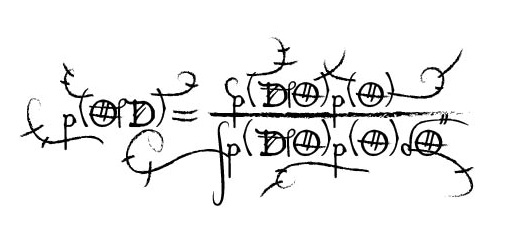
\includegraphics[width=1.5in]{Bayes.jpg}\hfil}\vfil}
%}

{
%\usebackgroundtemplate{\begin{center}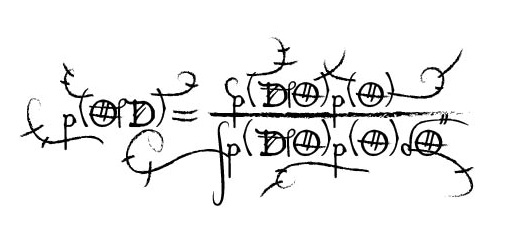
\includegraphics[width=0.4\paperwidth]{Bayes.jpg}\end{center}}
\usebackgroundtemplate{%
  \vbox to \paperheight{\hbox to \paperwidth{\hfil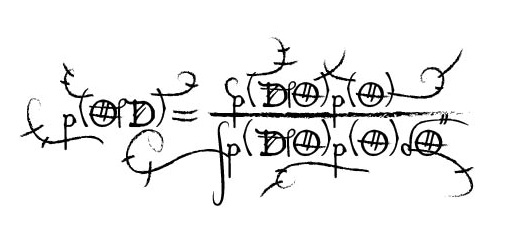
\includegraphics[width=2in]{Bayes.jpg}\hfil}}
}
\begin{frame}
\titlepage
\end{frame}
}
%\frame{\titlepage} 

%\frame{\frametitle{Overview of the talk}\tableofcontents}


\begin{frame}
\frametitle{Lecture overview}

\begin{itemize}
\item Bayesian variable selection
\bigskip
\item Model checking using posterior predictive
distribution

\end{itemize}

\end{frame}



\begin{frame}{Bayesian variable selection}

\begin{itemize}
\item Like \textbf{\color{blue}Hypothesis testing} (\textbf{\color{red}but fun}!).
\item \textbf{\color{blue}Linear regression}:
\[
y=\beta_{0}+\beta_{1}x_{1}+...+\beta_{p}x_{p}+\varepsilon.
\]
\item Which variables have \textbf{\color{red}non-zero} coefficient? Examples of hypotheses:
\begin{eqnarray*}
H_{0} & : & \beta_{0}=\beta_{1}=...=\beta_{p}=0\\
H_{1} & : & \beta_{1}=0\\
H_{2} & : & \beta_{1}=\beta_{2}=0
\end{eqnarray*}

\item Introduce \textbf{\textcolor{blue}{variable selection indicators}}
$\mathcal{I}=(\mathcal{I}_{1},...,\mathcal{I}_{p}).$ 
\item \textbf{\color{blue}Example} ($p=3$): $\mathcal{I}=(1,1,0)$ means that $\beta_{1}\neq0$ and $\beta_{2}\neq0$,
but $\beta_{3}=0$, so covariate $x_{3}$ drops out of the model.
\end{itemize}
\end{frame}

\begin{frame}{Bayesian variable selection, cont.}

\begin{itemize}
\item Crank the \textbf{\color{blue}Bayesian machine}:
\[
p(\mathcal{I}|y)\propto p(y|\mathcal{I}) p(\mathcal{I}).
\]%\medskip
\item \textbf{\color{blue}Note}: A \textbf{\color{red}probability distribution over models}. Model inference! \medskip
\item The prior $p(\mathbf{\mathcal{I}})$ is typically taken to be $\mathcal{I}_{1},...,\mathcal{I}_{p}|\theta\overset{iid}{\sim}\mathrm{Bernoulli}(\theta)$. \medskip
\item $\theta$ is the \textbf{\textcolor{blue}{prior inclusion probability}}.\medskip
\item \textbf{\color{blue}Note}: This prior "shrinks" the number of ''active'' parameters towards $p \theta$. \medskip
\item \textbf{\color{blue}Challenge}: Compute the \textbf{\textcolor{blue}{marginal likelihood}} \textrm{
for each model ($\mathcal{I}$)}
\[
p(y|\mathcal{I})=\int p(y|\beta,\mathcal{I})p(\beta|\mathbf{\mathcal{I}})d\beta.
\]

\end{itemize}
\end{frame}

\begin{frame}{Bayesian variable selection, cont.}

\begin{itemize}
\item Let $\beta_{\mathcal{I}}$ denote \textbf{\color{red}the subset of non-zero} coefficients
under $\mathcal{I}$. 
\item \textbf{\color{blue}Conjugate prior}:
\begin{align*}
\beta_{\mathcal{I}}|\sigma^{2} & \sim \mathcal{N}\left(0,\sigma^{2}\Omega_{\mathcal{I},0}^{-1}\right)\\
\sigma^{2} & \sim \text{Inv-}\chi^{2}\left(\nu_{0},\sigma_{0}^{2}\right).
\end{align*}

\item \textbf{\textcolor{blue}{Marginal likelihood}} (normal regression) 
\[
p(y| \mathbf{\mathcal{I}}) \propto \left|X_{\mathcal{I}}'X_{\mathcal{I}}+\Omega_{\mathcal{I},0}^{-1}\right|^{-1/2}\left|\Omega_{\mathcal{I},0}\right|^{1/2}\left(\nu_{0}\sigma_{0}^{2}+\mathrm{RSS}_{\mathcal{I}}\right)^{-(\nu_{0}+n-1)/2}.
\]
\item $X_{\mathcal{I}}$ is the \textbf{covariate matrix} for the subset given by $\mathcal{I}$.
\item $\Omega_{\mathcal{I}, 0}$ is (almost) the \textbf{prior precision} for the subset given by $\mathcal{I}$.
\item $\mathrm{RSS}_{\mathcal{I}}$ is (almost) the \textbf{residual sum of squares} under
model implied by $\mathbf{\mathcal{I}}$
\[
\mathrm{RSS}_{\mathcal{I}}=y'y-y'X_{\mathcal{I}}\left(X_{\mathcal{I}}'X_{\mathcal{I}}+\Omega_{\mathcal{I},0}\right)^{-1}X_{\mathcal{I}}'y.
\]

\end{itemize}
\end{frame}

\begin{frame}{Bayesian variable selection via Gibbs sampling}

\begin{itemize}
\item The \textbf{\color{blue}posterior} of the indicators $p(\mathcal{I}|y) \propto p(y|\mathcal{I})p(\mathcal{I})$...
\begin{itemize}
%\pause
\smallskip
\item ... is \textbf{\color{red}independent} of $\beta, \sigma^2$ [nothing but a \textbf{\color{blue}marginal likelihood}!]\smallskip
%\pause
\item ... $p(\mathcal{I}|y)$ is a \textbf{non-standard distribution}...\smallskip
\item ... includes a sample space with $2^p$ outcomes...\smallskip
%\pause
\item ... but the \textbf{\color{blue}full conditional} of a single $\mathcal{I}_j$ has two outcomes - \textbf{\color{red}Bernoulli}! \smallskip
\item ... how do we simulate $p(\mathcal{I}|y)$? \smallskip
\item \textbf{\color{blue}Gibbs sampling} to the rescue!
\end{itemize}
\smallskip
\item But the \textbf{outcome space} is still $2^p$ (huge!). \textbf{\color{blue}Example}: $$p=10\implies 2^{20}=1,048,576\quad \text{different models to explore...}$$ 
\item ... Don't I have to run the sampler for a \textbf{huge number} of iterations to \textbf{converge}?
\item Most of the $2^{p}$ models have \textbf{essentially zero probability}. We are saved!
\end{itemize}
\end{frame}


\begin{frame}
\frametitle{The Gibbs sampler for $\mathcal{I}$ in linear regression}
\begin{center}
\begin{minipage}{\columnwidth}
\begin{varblock}[0.95\columnwidth]{Gibbs sampling for $\mathcal{I}$ in  \textbf{\color{yellow}normal linear regression}}
Obtain $N$ samples from $p(\mathcal{I}|y)$ in the \textbf{\color{blue}linear regression} with \textbf{\color{blue}normal data} and \textbf{\color{blue}conjugate prior}.
\begin{itemize}
\item Set an (arbitrary) start point $$\mathcal{I}^{(0)}=(\mathcal{I}_1^{(0)}, \mathcal{I}_2^{(0)},  \dots, \mathcal{I}_p^{(0)}).$$
\item \textbf{For} $i=1,\dots, N$, 
\item[] ~~ \textbf{For} $j=1,\dots, p$,
\end{itemize}
\begin{enumerate}
\item[] ~~~~~~~ $\mathcal{I}_j^{(i)} \sim p(\mathcal{I}_j|\mathcal{I}_{-j}, y) = \mathrm{Bernoulli}(\theta_j)$,
$$\theta_j = \frac{p\left(y|\mathcal{I}_1^{(i)}, \dots ,\mathcal{I}_j = 1, \dots ,\mathcal{I}^{(i-1)}_p\right)p(\mathcal{I}_j=1)}{\sum_{m=0}^1 p\left(y|\mathcal{I}_1^{(i)}, \dots ,\mathcal{I}_j = m, \dots, \mathcal{I}^{(i-1)}_p\right)p(\mathcal{I}_j=m)}.$$
\item[] ~~ $\mathcal{I}^{(i)}=(\mathcal{I}_1^{(i)}, \mathcal{I}_2^{(i)}  \dots, \mathcal{I}_p^{(i)})$
\end{enumerate}
\end{varblock}
\end{minipage}
\end{center}

\end{frame}

\begin{frame}{The Gibbs sampler for $\mathcal{I}$ in linear regression, cont}

\begin{itemize}
\item Now we have $\{\mathcal{I}^{(i)}\}_{i=B}^N$ (\textbf{\color{blue}discard burn-in}, always!).
\item \textbf{But what about the parameters}? How do we sample $\beta$ and $\sigma^2$?
\item \textbf{\color{blue}Decompose} the joint posterior as usual
\[
p(\beta,\sigma^{2},\mathcal{I}|y)=p(\beta,\sigma^{2}|\mathcal{I},y)p(\mathcal{I}|y)=p(\beta|\sigma^{2},\mathcal{I},y)p(\sigma^{2}|\mathcal{I},y)p(\mathcal{I}|y).
\]
\vspace{-5mm}
\begin{center}
\begin{minipage}{\columnwidth}
\begin{varblock}[0.9\columnwidth]{Sample $\beta$ and $\sigma^2$ conditional on $\mathcal{I}$}
\begin{itemize}
\item \textbf{For} $i=B,\dots, N$, 
\begin{enumerate}
\item $\sigma^{2}|\mathcal{I}^{(i)},y, \sim \text{Inv-}\chi^{2}\left(\nu_{n},\sigma_{n}^{2}\right)$
\item \textrm{$\beta|\sigma^{2},\mathcal{I}^{(i)},y \sim \mathcal{N}\left(\mu_{n},\sigma^{2}\Omega_{n}^{-1}\right)$ }
\end{enumerate}
\item \textbf{\color{red}Note}: the \textbf{\color{blue}standard updates} for \textbf{linear regression with a conjugate prior} from  \textbf{\color{blue}Lecture 5}, but $\nu_n, \sigma_n^2, \mu_n, \Omega_n$ (and $\beta_0=0, \Omega_0$) all depend on $\mathcal{I}^{(i)}$.\\ \textbf{\color{blue}For example}:$$\mu_n = (X_{\mathcal{I}^{(i)}}'X_{\mathcal{I}^{(i)}} + \Omega_{0,\mathcal{I}^{(i)}})^{-1}X'_{\mathcal{I}^{(i)}}y.$$
\end{itemize}
\end{varblock}
\end{minipage}
\end{center}
\medskip
\item \textbf{\color{blue}Note}: \textbf{\color{red}Automatic model averaging} by integrating (by simulation) out the indicators!
\end{itemize}
\end{frame}


\begin{frame}{General Bayesian variable selection}

\begin{itemize}
\item The previous algorithm worked because the \textbf{\color{blue}marginal likelihood}
\[
p(y|\mathcal{I})=\int p(y|\beta, \sigma^2, \mathcal{I})p(\beta, \sigma^2| \mathcal{I})d\beta d\sigma^2
\]
was \textbf{\color{red}analytically tractable} [normal data and choice of prior].
\item \textbf{\color{blue}Bayesian variable selection} by \textbf{Metropolis-Hastings}: Markov chain in space $(\beta, \mathcal{I})$ to sample $p(\beta, \mathcal{I}|y)$ 
\item \textbf{\color{red}Note}: $\beta$ contains regression coefficients + other unknowns.
\item \textbf{\textcolor{blue}{Proposal for MH}} - \textbf{propose} $\beta$ and $\mathcal{I}$
jointly from
\[
q(\beta_{p}, \mathcal{I}_p | \beta_{c},\mathcal{I}_{c}) =  q_2(\beta_{p}|\beta_{c},\mathcal{I}_{p})q_1(\mathcal{I}_{p}|\mathcal{I}_{c}).
\]
\item \textbf{\color{blue}Main difficulty}: how to propose the \textbf{non-zero elements} in  $\beta_{p}$?
\item \textbf{\color{blue}Simple approaches}:
\begin{enumerate}
\item \textbf{Approximate posterior} with all variables in the model: $$\beta|y \overset{approx}{\sim} \mathcal{N}\left(\beta^{\star},J_{\beta^{\star},y}^{-1}\right).$$
\item Propose as in {\color{purple!75!black}1.} but \textbf{\color{blue}conditional on the zero restrictions} implied by $\mathcal{I}_{p}$.
Formulas are available (conditional of a multivariate normal is also normal).
\end{enumerate}
\end{itemize}
\end{frame}


\begin{frame}{Posterior predictive analysis}

\begin{itemize}
\item \textbf{\color{red}Idea}: If $p(y|\theta)$ is a 'good' model, then the data \textbf{\color{blue}actually observed} should not differ 'too much' from \textbf{\color{blue}simulated data} from $p(y|\theta)$.  \medskip
\item \textbf{\color{blue}Bayesian} ({\color{red}the joy of averaging}!): simulate data from \[
p(y^{\mathrm{rep}}|y)=\int p(y^{\mathrm{rep}}|\theta)p(\theta|y)d\theta \quad [\textbf{\textcolor{blue}{Posterior
predictive}}].
\]
\item \textbf{Difficult to compare} $y$ and $y^{\mathrm{rep}}$ because of \textbf{\color{blue}dimensionality}.\textbf{•}
\medskip
\item \textbf{\color{blue}Solution}: compare \textbf{\color{red}low-dimensional statistic} $T(y,\theta)$
to $T(y^{\mathrm{rep}},\theta)$. \medskip{}

\item \textbf{Evaluates} the \textbf{\color{blue}full probability model} consisting of \textbf{both} the likelihood \textit{and} prior distribution.
\end{itemize}
\end{frame}


\begin{frame}
\frametitle{Posterior predictive analysis, cont.}
\begin{center}
\begin{minipage}{\columnwidth}
\begin{varblock}[0.95\columnwidth]{Simulate from the \textbf{\color{yellow}posterior predictive density}
$p\left(T(y^{\mathrm{rep}})|y\right)$}
Obtain $N$ samples from $p\left(T(y^{\mathrm{rep}})|y\right)$.
\begin{itemize}
\item \textbf{For} $i=1,\dots, N$, 
\begin{enumerate}
\item Simulate a \textbf{\color{blue}parameter} $\theta^{(i)} \sim p(\theta|y)$.\smallskip
\item Simulate a \textbf{\color{blue}data-replicate} $y^{(i)}$ from $p(y^{\mathrm{rep}}|\theta^{(i)})$\smallskip.
\item $T^{(i)} = T(y^{(i)})$.
\end{enumerate}
\end{itemize}

\end{varblock}
\end{minipage}
\end{center}
\begin{itemize}
\item Compare the \textbf{\color{blue}observed statistic} $T(y)$ with the distribution
of $T(y^{rep})$ from our \textbf{\color{blue}simulation}. \smallskip
\item \textbf{\textcolor{blue}{Posterior predictive p-value}}: $$\Pr\left(T(y^{rep})\geq T(y)\right).$$ 
\item Informal \textbf{\color{blue}graphical analysis}.
\end{itemize}

\end{frame}


\begin{frame}{Posterior predictive analysis - Examples}

\begin{itemize}
\item \textbf{\color{blue}Example 1}: \textbf{Normal model}: $y_{1},...,y_{n}\overset{iid}{\sim}N(\mu,\sigma^{2})$.
$T(y)=\max_{i}\left|y_{i}\right|$.
\bigskip
\item \textbf{\color{blue}Example 2}: \textbf{ARIMA-process}. $T(y)$ may be the \textbf{autocorrelation function}.
\bigskip
\item \textbf{\color{blue}Example 3}: \textbf{Poisson regression}. $T(y)$ frequency distribution of the \textbf{response counts}. Or proportions of \textbf{zero counts}.
\end{itemize}
\end{frame}


\begin{frame}{Posterior predictive analysis - Normal model, max statistic}

\begin{figure}
\centering{}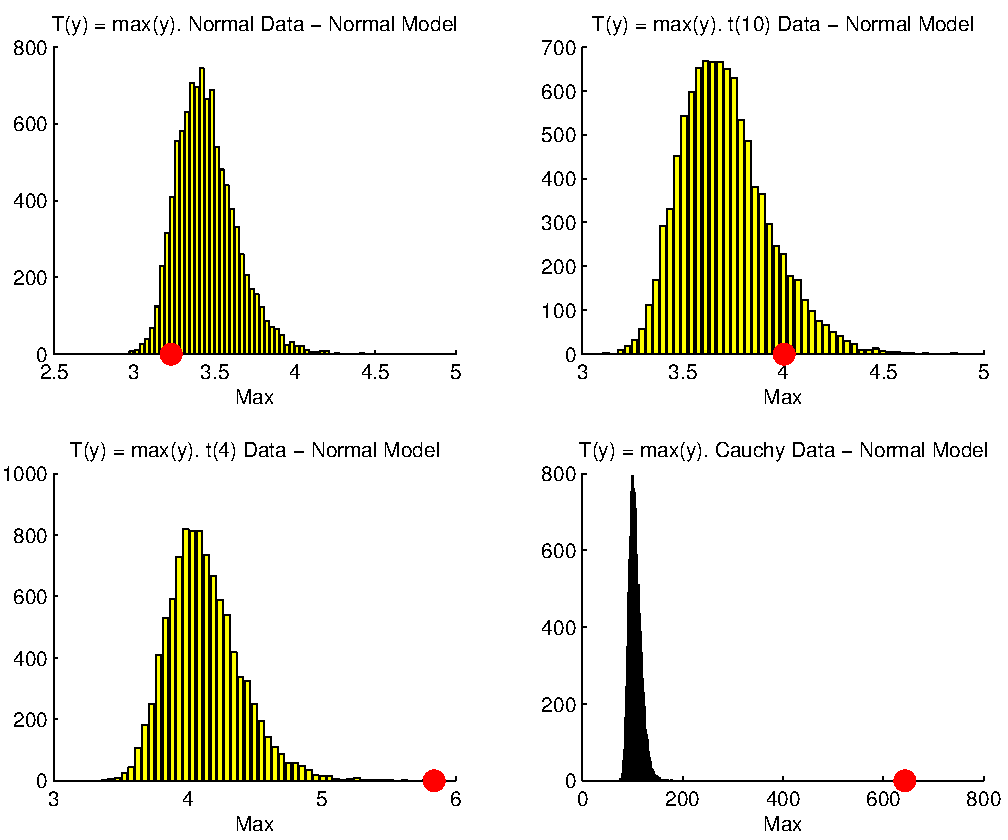
\includegraphics[scale=0.55]{PostPredNormalMaxStatistic}
\end{figure}


\end{frame}

\end{document}

